135. \begin{figure}[ht!]
\center{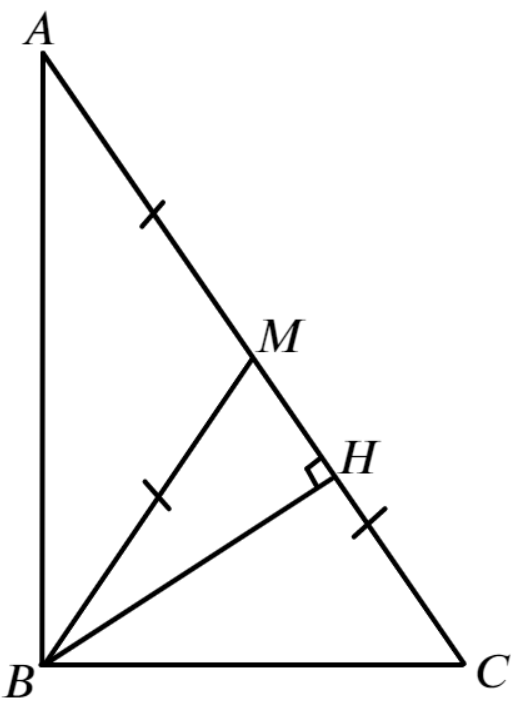
\includegraphics[scale=0.35]{g8-135.png}}
\end{figure}\\
Проведём медиану $BM$ и высоту $BH$ из прямого угла. Тогда $BM=\cfrac{1}{2}AC=\cfrac{1}{2}\cdot12=6$ и в прямоугольном треугольнике $BMH$ катет $BH$ в 2 раза меньше гипотенузы $BM,$ а значит $\angle BMH=30^\circ, \angle BMA=180^\circ-30^\circ=150^\circ.$ Треугольник $ABM$ является равнобедренным (так как медиана, проведённая из прямого угла, равна половине гипотенузы), значит $\angle B=(180^\circ-150^\circ):2=15^\circ,$ а тогда $\angle C=90^\circ-15^\circ=75^\circ.$\\
